\documentclass[border=10pt]{standalone}

\usepackage{tikz}
\usepackage{tikzsymbols}
\usetikzlibrary{calc,patterns,shapes.geometric}

\def\centerarc[#1](#2)(#3:#4:#5){\draw[#1] ($(#2)+({#5*cos(#3)},{#5*sin(#3)})$) arc (#3:#4:#5);}

\begin{document}
	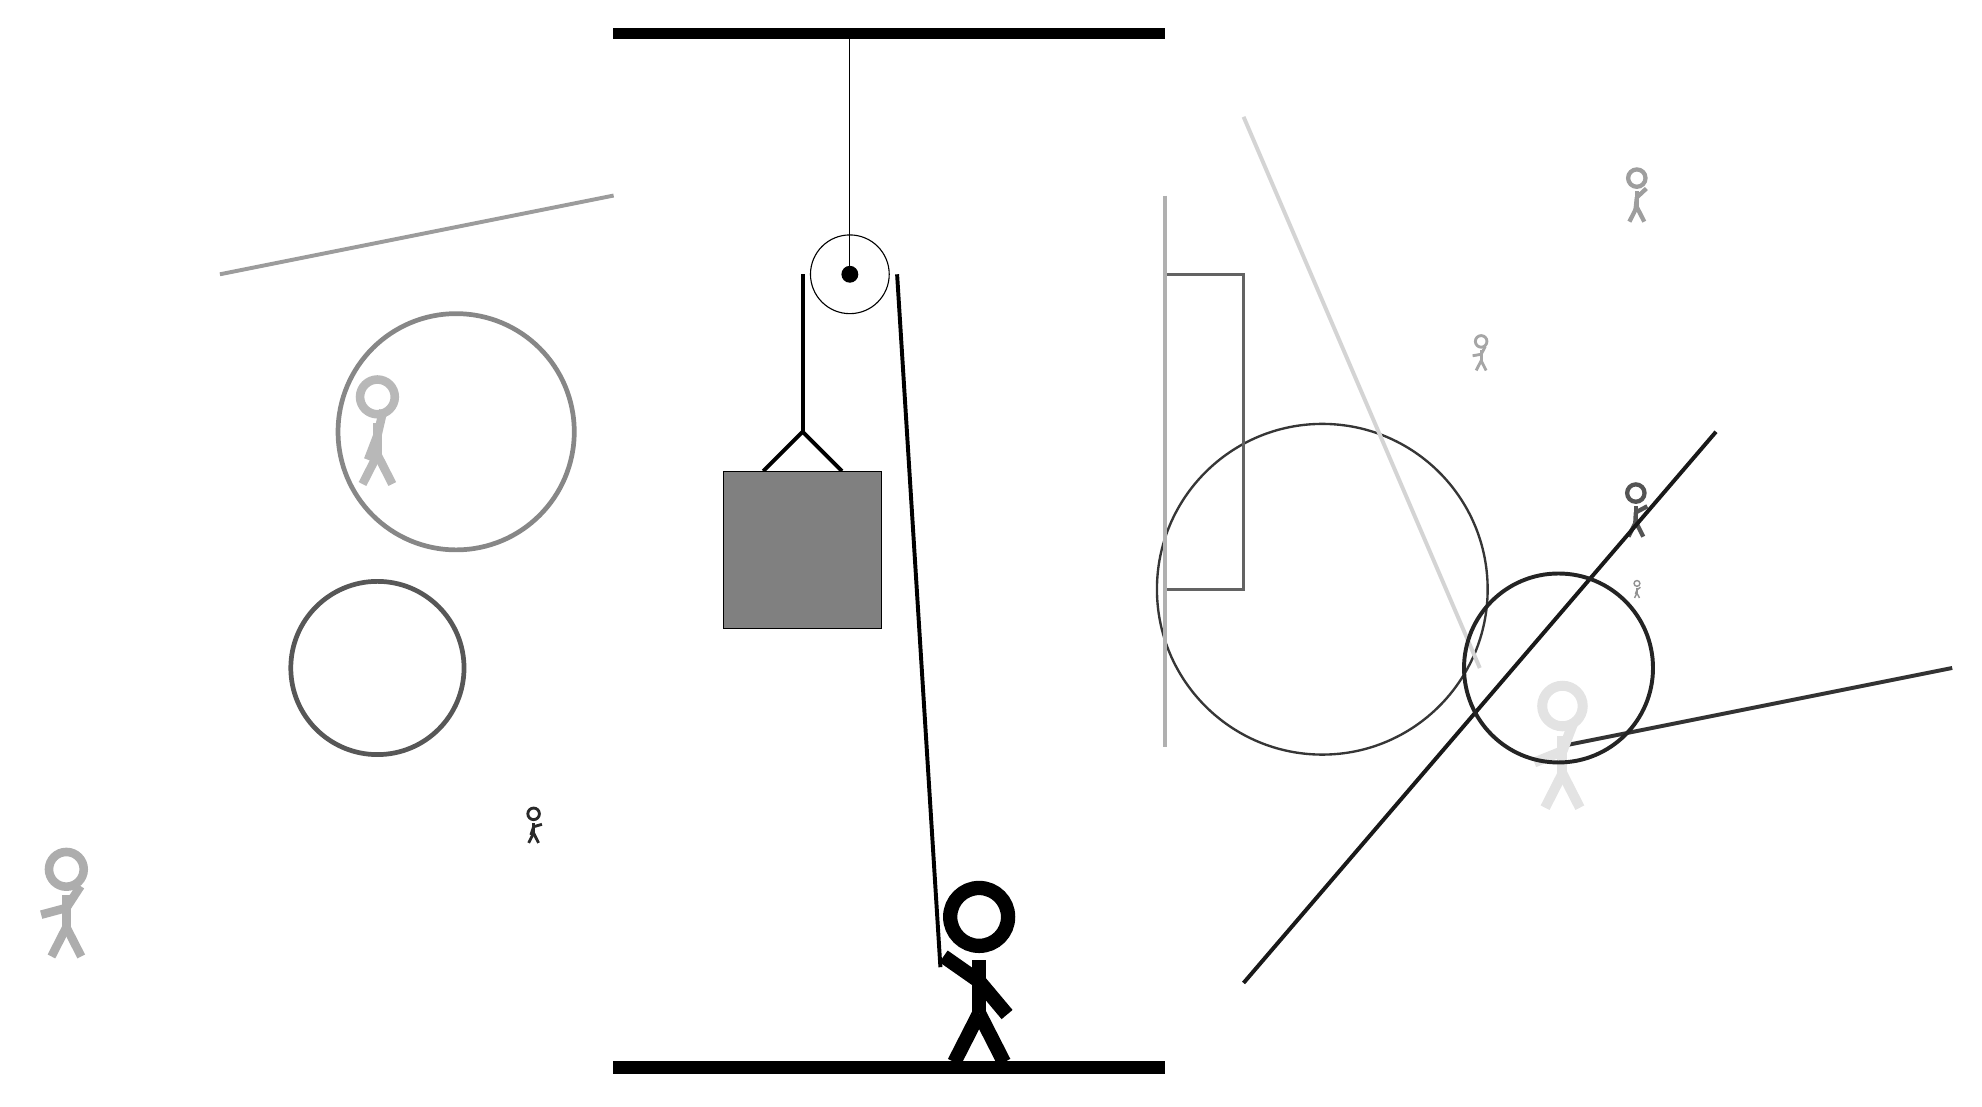
\begin{tikzpicture}
		%%%%% START %%%%%
		
		\draw[fill=black] (-2, 10) rectangle (5, 10.125);
		
		\draw (1, 7) circle (0.5);
		\draw[fill=black] (1, 7) circle (0.1);
		\draw (1, 10) -- (1, 7);
		
		\node[line width=0.5mm, color=black!67] at (11, 4) {\Strichmaxerl[3][87][28]};
		
		\draw[line width=0.4mm, color=black!32] (5, 4) rectangle (5, 3);
		\draw [line width=0.3mm, color=black!79](7, 3) circle (2.1);
		\draw [line width=0.6mm, color=black!66](-5, 2) circle (1.1);
		
		\draw[line width=0.5mm, color=black!90](6, -2) -- (12, 5);
		\draw[line width=0.5mm, color=black!17](6, 9) -- (9, 2);
		\node[line width=0.2mm, color=black!32] at (-9, -1) {\Strichmaxerl[6][15][57]};
		\node[line width=0.3mm, color=black!84] at (-3, 0) {\Strichmaxerl[2][72][16]};
		\draw[line width=0.4mm, color=black!61] (5, 7) rectangle (6, 3);
		\node[line width=0.5mm, color=black!38] at (11, 8) {\Strichmaxerl[3][84][43]};
		\node[line width=0.3mm, color=black!35] at (9, 6) {\Strichmaxerl[2][10][62]};
		
		\draw[line width=0.5mm, color=black!52] (5, 3) rectangle (5, 7);
		\draw [line width=0.6mm, color=black!47](-4, 5) circle (1.5);
		\node[line width=0.7mm, color=black!43] at (11, 3) {\Strichmaxerl[1][69][37]};
		\draw[line width=0.5mm, color=black!80](10, 1) -- (15, 2);
		\node[line width=0.3mm, color=black!28] at (-5, 5) {\Strichmaxerl[6][69][77]};
		\node[line width=0.6mm, color=black!11] at (10, 1) {\Strichmaxerl[7][22][69]};
		\draw [line width=0.5mm, color=black!86](10, 2) circle (1.2);
		\draw[line width=0.5mm, color=black!39](-7, 7) -- (-2, 8);
		\draw[line width=0.5mm, color=black!31](5, 8) -- (5, 1);
		
		\draw[line width=0.5mm] (-0.1, 4.5) -- (0.4, 5.0) -- (0.9, 4.5);
		\draw[fill=black!50] (-0.6, 4.5) rectangle (1.4, 2.5);
		
		\draw[line width=0.5mm] (0.4, 7) -- (0.4, 5.0);
		\centerarc[line width=0.5mm](1, 7)(0:180:0.6);
		\draw[line width=0.5mm](1.6, 7) -- (2.15, -1.8);
		
		\node at (2.6, -1.9) {\Strichmaxerl[10][-35][-50]};
		
		\draw[fill=black] (-2, -3) rectangle (5, -3.15);
		
		%%%%% END %%%%%
	\end{tikzpicture}
\end{document}